\chapter{Ist-Analyse ( 5 \%)}
\label{chap:ist-analyse}

Dieses Kapitel dient der Beschreibung existierender System.
Es soll ihre Eigenschaften und Probleme aufzeigen.
Diese werden zuerst Theoretisch betrachtet und
dann an Systemen in der Praxis demonstriert.

% dieses kap dient .. und damit soll .. aufbau

\section{Eigenschaften der existierenden Systeme}

\subsection{Struktur}
Wie in der folgenden Grafik leicht zu erkennen,
sind traditionellen CI-Systeme Client-Server Systeme.

\begin{figure}[ht]
  \centering
  \label{fig:ist-aufbau-tradition}
  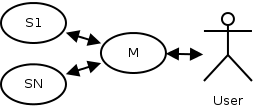
\includegraphics[height=1in]{imageinput/ist-aufbau-tradition.png}
  \caption{Logischer Aufbau eines CI System}
\end{figure}

Der sogenannte Master ist der Server und verwaltet alle Daten.
Die Slaves sind die Clients und verrichten die eigentliche Arbeit.
Sie sammeln Daten und liefern diese einschliesslich der Resultate beim Master ab.

Benutzer interagieren Ausschliesslich mit dem Master.

\subsection{Datensammlung}
Wie bereits in Sektion~\ref{sec:base:ci} erw\"ahnt,
f\"uhrt ein CI-System nicht nur Auftr\"age aus,
sondern sammelt auch daten f\"ur die sp\"atere Weiterverarbeitung.

Die Datensammlung l\"asst sich dabei grob in 2 Bereiche einteilen.
Zum einen die Laufzeitdaten und zum anderen die Artefakte.

Laufeitdaten fallen bereits w\"ahrend der Ausf\"uhrung an,
und beinhalten in der Regel zumindest die Textuellen Ausgaben
der ausgef\"uhrten Programme.
Weitere M\"oglichkeiten k\"onnen Testresultate, echzeit Logs und Ausf\"uhrungsstatistiken sein.
Laufzeitdaten werden dem Benutzer in idr. Zeitnah zur Verf\"ugung gestellt.

Artefakte hingegen sind Dateien,
welche erst nach Abschluss eines Schrittes zur verf\"ugung stehen.
Zu ihnen gehoeren neben den traditionellen ausf\"uhrbaren Dateien
auch lauff\"ahige Archive des Gesammtprogrammes oder Testergebnisse in den Formaten JunitXML oder TAP.

%XXX: cite tap, junitxml

Diese werden zum Master geschickt, dort aufbewahrt und sp\"ater genutzt.

In der Regel werden ausf\"uhrbare Artefakte zum Download angeboten,
w\"ahrend Testergebnisse nur dargestellt werden.





\section{Probleme existierender Systeme}

Diese Sektion gibt einen \"Uberblick \"uber die Problemarten

\subsection{Datenzugriff}

Beim Datenzugriff sind die existierenden Systeme besonders Problematisch.
Es gibt Grunds\"atzlich keinerlei Standardschnittstellen.
Die meisten Systeme verwenden noch nicht einmal eine Datenbank.
Jene welche doch eine verwenden wird, machen sie nicht zug\"anglich.

Die Datenhaltung dieser Systeme kann somit grob als geordnete Ablage klassifiziert werden. Weiterf\"uhrende Abfragen sind nicht m\"oglich.

\subsection{Erweiterbarkeit}

Die Erweiterbarkeit eines CI-Systemes wird von 2 Hauptpunkten dominiert.
Dies ist die Integration in die Benutzeroberfl\"ache
und zum anderen die M\"oglichkeiten mit den Daten interagieren
und auf neue Weise zu kombinieren.

Die erweiterbaren Systeme stellen normalerweise zumindest eine Schnittstelle
f\"ur die graphische Oberfl\"ache zur Verf\"ugung.
Damit ist zumindest das problemlose Anpassen der Benutzerschnittstelle gegeben.


%XXX:


\subsection{Komponentenabh\"angigkeit}

Wie bereits in Kapitel~\ref{25d}

\begin{verbatim}
  - strikt master/slave
  - client/server prob
  - zentrales management
  - alles wird im master gemanagt
  - dumme arbeiter, keinerlei autonomie

  - ausfall von master bedingt ausfall von slave


\end{verbatim}

\section{Praxisbeispiele}

Um Probleme in der Praxis aufzuzeigen,
soll eine Auswahl and Werzeugen getroffen werden.
Anschliessend werden ihre Eigenschaften und Probleme n\"aher untersucht.


\subsection{Auswahl}




\begin{verbatim}

- opensource/oeffentlich
- kostenlos
- verbreitet

\end{verbatim}

\subsection{Jenkins}

\begin{verbatim}
pro:
- build matrix
- ui

cons:
- datenzugriff
- erweiterungen
- dateninteraktion?

\end{verbatim}

%XXX referenzen
Jenkins und Hudson stellen ein Benutzerfreundliches,
jedoch limitiertes System zum einfachen Anlegen von Build-Jobs.

Parametrisierung ist nicht möglich.

\subsection{Buildbot}


\begin{verbatim}


\cite auf meinen versuch

pro:
- flexible builds
- rudimentaerer datenzugriff
- parameter (z.b. branch)
cons:
- datenmodell
- ui


- beispiel pypy uebersicht

\end{verbatim}


%XXX referenzen
BuildBot positioniert sich als eine Art Meta-Build-Server.
es biete keine normale Oberfläche, sondern wird mittels
Komposition von Metadaten und Komponenten konfiguriert.

Die Konfiguration des Servers stellt dabei ein Python script,
welches die Operationen ausführt, welche zur Zusammenstellung des gewünschten Servers notwendig sind.

Es ist möglich Builds Jobs mit minimale Parameter in Form von Strings zu Übergeben.

\subsection{TravisCI}

\begin{verbatim}
pro:
- ui
  - screenshoot
- matix builds
- branch builds -> via pull req

cons
- mangel an datenzugriff
- hosted
- nicht portabel
\end{verbatim}



\section{Zusammenfassung}

% Dieses Kap. hat getz ..

% wie haben gesehen das ..

% im folgenden verlauf der arbeit \ldots
% 2-3 saetze
